\paragraph{QuizziPedia::Front-End::Services::AuthService}
\begin{figure}[ht]
	\centering
	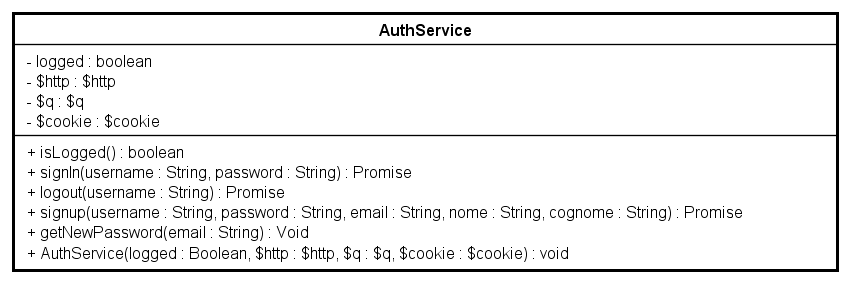
\includegraphics[scale=0.80]{UML/Classi/Front-End/QuizziPedia_Front-end_Services_AuthService.png}
	\caption{QuizziPedia::Front-End::Services::AuthService}
\end{figure} \FloatBarrier
\begin{itemize}
	\item \textbf{Descrizione}: questa classe permette di gestire la registrazione e l'autenticazione di un utente;
	\item \textbf{Utilizzo}: fornisce le funzionalità di registrazione e autenticazione ai controllers. Controlla che i dati inseriti dall'utente siano presenti nel \textit{Database\ped{G}} in caso di autenticazione. Presenta anche le funzionalità per la gestione del reset della password;
	\item \textbf{Relazione con altre classi:}
	\begin{itemize}
		\item \textbf{OUT \texttt{LoginController}}: questa classe gestisce la logica alla base della pagina di autenticazione;
		\item \textbf{OUT \texttt{PasswordForgotController}}: questa classe gestisce la logica alla base del reset della password;
		\item \textbf{OUT \texttt{SignUpController}}: questa classe gestisce la logica alla base della registrazione di un nuovo utente.
	\end{itemize}
	\item \textbf{Attributi}:
	\begin{itemize}
		\item \texttt{-} \texttt{logged: Boolean} \\ Campo dati che indica se l'utente è autenticato;
		\item \texttt{-} \texttt{\$http: \$http} \\ Campo dati che contiene un riferimento al servizio \$http che permette la comunicazione con il protocollo \textit{HTTP\ped{G}};
		\item \texttt{-} \texttt{\$q: \$q} \\ Campo dati che contiene un riferimento a \$q, un servizio offerto da \textit{AngularJS\ped{G}} per la gestione, tramite \textit{Promise\ped{G}}, di chiamate asincrone;
		\item \texttt{-} \texttt{\$cookie: \$cookie} \\ Campo dati che consente di salvare il valore di logged ed evitare che venga richiesta l'autenticazione ad ogni ricaricamento della pagina.
	\end{itemize}
	\item \textbf{Metodi}:
	\begin{itemize}
		\item \texttt{+} \texttt{AuthService(logged: Boolean, \$http: \$http, \$q: \$q, \$cookie: \$cookie)} \\ Metodo costruttore della classe; \\
		\textbf{Parametri}:
		\begin{itemize}
			\item \texttt{logged: Boolean} \\ Parametro che indica se l'utente è loggato o no;
			\item \texttt{\$http: \$http} \\ Parametro contenente un riferimento al servizio \$http creato da \textit{AngularJS\ped{G}} per facilitare la comunicazione mediante protocollo \textit{HTTP\ped{G}};
			\item \texttt{\$q: \$q} \\ Parametro contenente un riferimento al servizio \$q creato da \textit{AngularJS\ped{G}} per facilitare la gestione di funzione asincrone mediante l’utilizzo delle \textit{Promise\ped{G}};
			\item \texttt{\$cookie: \$cookie} \\ Parametro che consente di salvare il valore di logged ed evitare che venga richiesta l'autenticazione ad ogni ricaricamento della pagina.
		\end{itemize}
		\item \texttt{+} \texttt{isLogged(): Boolean} \\ Metodo che restituisce il valore dell'attributo \textit{logged} salvato all'interno del cookie che permette di evitare di eseguire l'autenticazione ad ogni caricamento della pagina;
		 
		\item \texttt{+} \texttt{signIn(email: String, password: String): Promise}\\ Metodo che permette di effettuare il login all'applicazione facendo una richiesta di autenticazione al back-end passando i parametri ricevuti. Il metodo ritorna una \textit{Promise\ped{G}}. In caso la \textit{Promise\ped{G}} venga rifiutata, verrà restituito al \texttt{LoginController} un oggetto \texttt{ErrorModelInfo} contenente tutti i dettagli dell'errore. In caso la \textit{Promise\ped{G}} venga accettata, verrà restituito al chiamante del metodo il risultato della chiamata; \\
			\textbf{Parametri}: 
			\begin{itemize}
				\item \texttt{username: String} \\ Parametro che rappresenta lo username o la email dell'utente;
				\item \texttt{password: String} \\ Parametro che rappresenta la password dell'utente.
			\end{itemize}
			
		\item \texttt{+} \texttt{logout(username: String): Promise} \\ Metodo che permette di effettuare il logout dall'applicazione. Il metodo ritorna una \textit{Promise\ped{G}}. In caso la \textit{Promise\ped{G}} venga rifiutata, verrà restituito al \texttt{LogoutController} un oggetto \texttt{ErrorModelInfo} contenente tutti i dettagli dell'errore. In caso la \textit{Promise\ped{G}} venga accettata, verrà restituito al chiamante del metodo il risultato della chiamata.\\
		\textbf{Parametri}:
		\begin{itemize}
			\item \texttt{username: String} \\ Parametro che rappresenta l'utente che vuole eseguire il logout.
		\end{itemize}
		
		\item \texttt{+} \texttt{signup(username: String, password: String, email: String, nome: String, cognome: String): Promise} \\Metodo che permette di effettuare la registrazione all'applicazione tramite richiesta di creazione nuovo account al back-end. Il metodo ritorna una \textit{Promise\ped{G}}. In caso la \textit{Promise\ped{G}} venga rifiutata, verrà restituito al \texttt{SignUpController} un oggetto \texttt{ErrorModelInfo} contenente tutti i dettagli dell'errore. In caso la \textit{Promise\ped{G}} venga accettata, verrà restituito al chiamante del metodo il risultato della chiamata; \\
			\textbf{Parametri}:
			\begin{itemize}
				\item \texttt{username: String} \\ Parametro che rappresenta lo username o la email dell'utente;
				\item \texttt{password: String} \\ Parametro che rappresenta la password dell'utente;
				\item \texttt{email: String} \\ Parametro che rappresenta la email dell'utente;
				\item \texttt{nome: String} \\ Parametro che rappresenta il nome dell'utente;
				\item \texttt{cognome: String} \\ Parametro che rappresenta il cognome dell'utente.
			\end{itemize}
			
		\item \texttt{+} \texttt{getNewPassword(email: String): Void}  \\Metodo che permette il recupero della password. Il metodo ritorna una \textit{Promise\ped{G}}. In caso la \textit{Promise\ped{G}} venga rifiutata, verrà restituito al \texttt{PasswordForgotController} un oggetto \texttt{ErrorModelInfo} contenente tutti i dettagli dell'errore. In caso la \textit{Promise\ped{G}} venga accettata, verrà restituito al chiamante del metodo il risultato della chiamata. \\
			\textbf{Parametri}:
			\begin{itemize}
				\item \texttt{email: String} \\ Parametro che rappresenta la email a cui mandare un messaggio per resettare la password.
			\end{itemize}
	\end{itemize}
\end{itemize}